%%%%%%%%%%%%%%%%%%%%%%%%%%%%%%%%%%%%%
% Read the /ReadMeFirst/ReadMeFirst.tex for an introduction. Check out the accompanying book "Better Books with LaTeX the Agile Way" for a discussion of the template and step-by-step instructions. The template was originally created by Clemens Lode, LODE Publishing (www.lode.de), mail@lode.de, 8/17/2018. Feel free to use this template for your book project!
%%%%%%%%%%%%%%%%%%%%%%%%%%%%%%%%%%%%%

% Replace Replace with First Chapter Name
% Replace p1_firstchapter:cha with your chapter title label (no spaces, only lower case letters)
% Replace the text below \end{chapterpage} and insert your own text.

%\begin{chapterpage}{Foundations}{p1_firstchapter:cha}

%\begin{myquotation} The perfect place for an introducing quotation.\par\vspace*{15mm}
%\mbox{}\hfill \emdash{}Famous Person\index{Person, Famous}
%, \citetitle{bibitem}\index{@\citetitle{bibitem}} %\ifxetex\label{famousperson-bibitem-quote}\else\citep[p.~123]{bibitem}\fi
%\par\end{myquotation}

%\end{chapterpage}

% -------------------- replace or remove text below and paste your own text ------

\chapter{Extending into the Wilds}\label{c1}

sdfsfsfd

\section{Equations and Stuff}\label{c1basicformatting:sec}

$e = mc^2$

\begin{equation}
e^{i\pi}=-1 
\end{equation}

\begin{figure}
\tikzsetnextfilename{equation1}
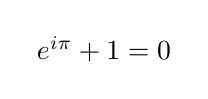
\begin{tikzpicture}
    \node at (0,0) {$e^{i\pi} + 1 = 0$};
\end{tikzpicture}
\end{figure}

\begin{minted}[
frame=lines,
framesep=5mm,
baselinestretch=0.9,
bgcolor=LightGray,
fontsize=\footnotesize,
linenos,
mathescape
]{python}
	import numpy as np
	     
	def incmatrix(genl1,genl2):
	    m = len(genl1)
	    n = len(genl2)
	    M = None #to become the incidence matrix
	    VT = np.zeros((n*m,1), int)  #dummy variable
	    
	    #compute the bitwise xor matrix $e=mc^2$
	    M1 = bitxormatrix(genl1)
	    M2 = np.triu(bitxormatrix(genl2),1) 
	
	    for i in range(m-1):
	        for j in range(i+1, m):
	            [r,c] = np.where(M2 == M1[i,j])
	            for k in range(len(r)):
	                VT[(i)*n + r[k]] = 1;
	                VT[(i)*n + c[k]] = 1;
	                VT[(j)*n + r[k]] = 1;
	                VT[(j)*n + c[k]] = 1;
	                
	                if M is None:
	                    M = np.copy(VT)
	                else:
	                    M = np.concatenate((M, VT), 1)
	                
	                VT = np.zeros((n*m,1), int)
	    
	    return M
\end{minted}


    \begin{figure}
        \tikzsetnextfilename{flower}
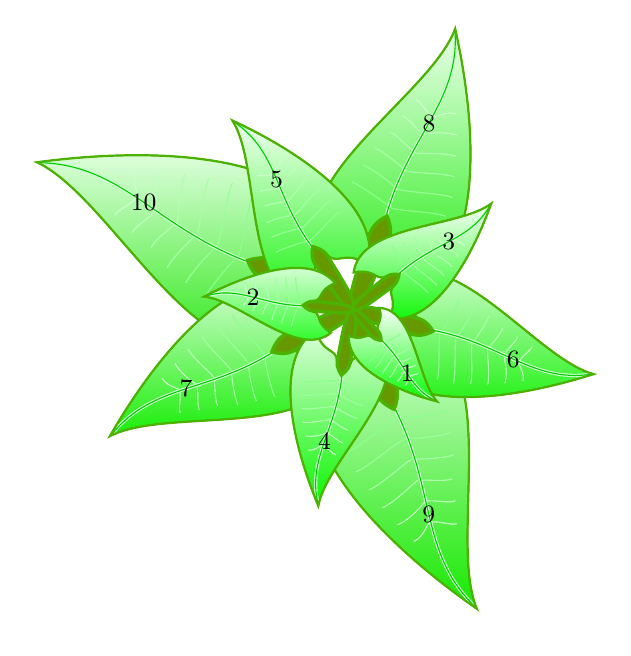
\begin{tikzpicture}

\foreach \x in {10,...,1}
{\draw[shade,bottom color=red!\x!green,top color=green!\x,x=0.3 pt,y=0.3 pt,scale={0.4+0.1*\x},rotate=222.5*\x] (0,0) .. 
controls ( -11,  1) and ( -9, 50) .. (-10,80) ..
controls ( -16, 60) and (-32, 75) .. (-50,40) .. 
controls (-110,100) and (-0,230) ..  (  0,300)  node[below] (\x) {} ..
controls (  45,230) and (110,100) .. ( 50,40) ..
controls (  32, 75) and ( 16, 60) ..  ( 10,80) ..
controls (   9, 50) and ( 11,  1) .. (  0,0) 
-- cycle ;

\draw[thin,green!45,x=0.3 pt,y=0.3 pt,scale={0.4+0.1*\x},rotate=222.5*\x] (-45,120) .. controls (-35,120) and (0,110) .. (-3,110) .. controls (0,105) and (40,120) .. (55,120);
\draw[thin,green!40,x=0.3 pt,y=0.3 pt,scale={0.4+0.1*\x},rotate=222.5*\x] (-40,140) .. controls (-30,140) and (0,130) .. (-3,130) .. controls (0,125) and (40,140) .. (55,140);
\draw[thin,green!35,x=0.3 pt,y=0.3 pt,scale={0.4+0.1*\x},rotate=222.5*\x] (-35,160) .. controls (-25,160) and (0,150) .. (0,150) .. controls (0,145) and (35,160) .. (50,160);
\draw[thin,green!30,x=0.3 pt,y=0.3 pt,scale={0.4+0.1*\x},rotate=222.5*\x] (-25,180) .. controls (-17,180) and (0,170) .. (3,170) .. controls (0,165) and (30,180) .. (45,180);
\draw[thin,green!25,x=0.3 pt,y=0.3 pt,scale={0.4+0.1*\x},rotate=222.5*\x] (-20,200) .. controls (-13,200) and (0,190) .. (6,190) .. controls (0,185) and (20,200) .. (38,200);
\draw[thin,green!20,x=0.3 pt,y=0.3 pt,scale={0.4+0.1*\x},rotate=222.5*\x] (-13,220) .. controls (-8,220) and (3,210) .. (8,210) .. controls (10,205) and (18,220) .. (30,220);
\draw[very thick,green!20,x=0.3 pt,y=0.3 pt,scale={0.4+0.1*\x},rotate=222.5*\x] (0,90) .. controls (-10,180) and (30,230) .. (1,297);
\draw[thin,black!20!green,x=0.3 pt,y=0.3 pt,scale={0.4+0.1*\x},rotate=222.5*\x] (0,90)  .. controls (-10,180) and (30,230)  .. (1,297) node[midway,black] (num\x) {\small\x};
\draw[very thick,red!30!green,fill=red!40!green,x=0.3 pt,y=0.3 pt,scale={0.4+0.1*\x},rotate=222.5*\x] 
(0,0) .. 
controls ( -11,  1) and ( -9, 50) ..
(-10,80) .. 
controls (-10,90) and (0,100) .. (0,100) ..
controls (0,100) and (10,90) .. (10,80)..
controls (   9, 50) and ( 11,  1) .. (  0,0) 
-- cycle;
\draw[thick,red!30!green,x=0.3 pt,y=0.3 pt,scale={0.4+0.1*\x},rotate=222.5*\x] (0,0) .. 
controls ( -11,  1) and ( -9, 50) .. (-10,80) ..
controls ( -16, 60) and (-32, 75) .. (-50,40) .. 
controls (-110,100) and (-0,230) ..  (  0,300) ..
controls (  45,230) and (110,100) .. ( 50,40) ..
controls (  32, 75) and ( 16, 60) ..  ( 10,80) ..
controls (   9, 50) and ( 11,  1) .. (  0,0) 
-- cycle ;
}
%\draw[->,>=latex,x=0.3 pt,y=0.3 pt,black] ([xshift=6pt] 8.east) arc (69:-69:350) node[midway,right] {} };
\end{tikzpicture}
    \end{figure}


    \begin{figure}
        \tikzsetnextfilename{my_externalized_plot}
	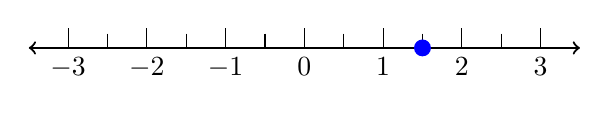
\begin{tikzpicture}
	         \foreach \x in {-3,...,3} {
	            \draw(\x,0.25) --(\x,0)node[below]{$\x$};
	          }
	          \foreach \x in {-2.5,...,2.5} {
	            \draw(\x,0.18) --(\x,0);
	          }
	          \draw[thick,<->](-3.5,0)--(3.5,0);
	          \filldraw[blue](1.5,0) circle (1mm);
	\end{tikzpicture}

-3 -2 -1 0 1 2 3
    \end{figure}

% Here we specify the figure will be converted and inserted as PNG
        \tikzsetnextfilename{circle}
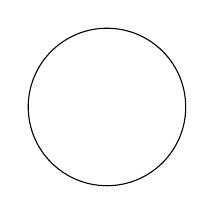
\begin{tikzpicture}
    \draw (0,0) circle (1) ;
\end{tikzpicture}